\section{Testing}
\label{sec:testresult}

One of the key tasks that have been planned in this project was testing. In
section \ref{sec:testing}, a detailed purpose, plan and focus of our testing
strategy has been outlined. Having finished the prototype, it is very important
that each requirements were tested to make sure that no functionality
misbehaves or fails to perform as expected. Each of the nine requirements were
tested and the test results are documented in this section. This section
somewhat describes what has happened with the pilot prototype, a number of
modification have been incorporated as the testing went on to correct defects.
Several tests have been conducted on each functionality and code section during
the sprints, but this section is the final test result documentation that
declares each requirement as either working or not working.

The result of usability testing is also included as part of this section. The
usability test section tries to show how our prototype fared in the user space
of actual Artsdatabanken users. It gives a preview of how the application has
been received, criticized and modification prompts that arise from users.

\subsection{Functionality test results}

\newpage
\subsection*{Test 1 (run 1)}

	\begin{table}[htb]
		\centering
		\begin{tabular}{|p{3.5cm}|p{7.0cm}|} \hline
			\textbf{Requirements} & F1 and F10 \\ \hline
			\textbf{Version} & 0.9 \\ \hline
			\textbf{Date} & 2011-11-02 \\ \hline
			\textbf{Tested by} & Stian Liknes \\ \hline
			\textbf{Test environment} & Sony Ericsson Xperia X10 running Android 2.1.1.A.0.6 with kernel: 2.6.29 \\ \hline
			\textbf{Pre-conditions} & Clean install of app on mobile device, no observations stored \\ \hline
			\textbf{Post-conditions} & A new observation has been saved and the user is directed back to the main menu \\ \hline
			\textbf{Result} & PASS \\ \hline
			\textbf{Comments} & Could only choose GPS coordinates in step 3, close locations missing \\ \hline
		\end{tabular}
		\caption{Summary of test 1}
	\end{table}

	\begin{table}[htb]
		\centering
		\begin{tabular}{|p{5.0cm}|p{5.0cm}|p{1cm}|}
			\hline \textbf{Action} & \textbf{Expected outcome} & \textbf{Result} \\ \hline
			1. Tap the new observation button & Menu for selecting species group appears & PASS \\ \hline
			2. Select species type "Fugl" (bird) & Menu for bird observations appears & PASS \\ \hline
			3. Selects location from list of close locations, or selects GPS location & Location is set & PASS \\ \hline
			4. Start writing "grågås" in the "Art" (species) field, ensure that
			auto-complete give useful suggestions, choose "grågås" from list of
			suggestions. Write 2 in the "Antall" (count) field & Auto-complete
			suggests bird names, 2 species of type "grågås" is added to observation
			& PASS \\ \hline 
			5. Tap "Lagre". & Observatin is saved & PASS \\ \hline
		\end{tabular}
		\caption{Execution of test 1}
	\end{table}

\newpage
\subsection*{Test 2 (run 1)}

	\begin{table}[htb]
		\centering
		\begin{tabular}{|p{3.5cm}|p{7.0cm}|} \hline
			\textbf{Requirement} & F2 \\ \hline
			\textbf{Version} & 0.9 \\ \hline
			\textbf{Date} & 2011-11-02 \\ \hline
			\textbf{Tested by} & Stian Liknes \\ \hline
			\textbf{Test environment} & Sony Ericsson Xperia X10 running Android 2.1.1.A.0.6 with kernel: 2.6.29 \\ \hline
			\textbf{Pre-conditions} & Test 1 completed in same test environment, app is still in observation view \\ \hline
			\textbf{Post-conditions} & Additional information about an observation has been saved \\ \hline
			\textbf{Result} & PASS \\ \hline
		\end{tabular}
		\caption{Summary of test 2}
	\end{table}

	\begin{table}[htb]
		\centering

		\begin{tabular}{|p{5.0cm}|p{5.0cm}|p{1cm}|}
			\hline \textbf{Action} & \textbf{Expected outcome} & \textbf{Result} \\ \hline

			1. Tap "Detaljer" (details) in the row containing "grågås" &
			Detailed view for the "grågås" observation is displayed & 
			PASS \\ \hline

			2. Select "Rugende" in the "Aktivitet" (activity) field &
			"Aktivitet" field populated with "Rugende" &
			PASS \\ \hline

			3. Tap back button & 
			Main observation view is displayed & 
			PASS \\ \hline

			4. Tap save and go to main screen. Go into the observatin using
			"Lagrede Observasjoner" (stored observations) and verify that "grågås"
			still has "Aktivitet" set to "Rugende" in the details view &
			Grågås has "Aktivitet" set to "Rugende" &
			PASS \\ \hline
		\end{tabular}
		\caption{Execution of test 2}
	\end{table}

\newpage
\subsection*{Test 3 (run 1)}

	\begin{table}[htb]
		\centering
		\begin{tabular}{|p{3.5cm}|p{7.0cm}|} \hline
			\textbf{Requirement} & F3 \\ \hline
			\textbf{Version} & 0.9 \\ \hline
			\textbf{Date} & 2011-11-02 \\ \hline
			\textbf{Tested by} & Stian Liknes \\ \hline
			\textbf{Test environment} & Sony Ericsson Xperia X10 running Android 2.1.1.A.0.6 with kernel: 2.6.29 \\ \hline
			\textbf{Pre-conditions} & Test 1 completed in same test environment, app is still in observation view \\ \hline
			\textbf{Post-conditions} & Observation is stored with two entries, "grågås" ("Antall" of 2) and "blåmeis" ("Antall" of 1) \\ \hline
			\textbf{Result} & FAIL \\ \hline
			\textbf{Comments} & Could not perform step 2, no place to select different locations \\ \hline
		\end{tabular}
		\caption{Summary of test 3}
	\end{table}

	\begin{table}[htb]
		\centering
		\begin{tabular}{|p{5.0cm}|p{5.0cm}|p{1cm}|}
			\hline \textbf{Action} & \textbf{Expected outcome} & \textbf{Result} \\ \hline

			1. Tap "Legg til ny art" &
			A empty species row is appended &
			PASS \\ \hline
			
			2. Optionally selects another location, otherwise the same one is
			selected. & 
			New location chosen for current row &
			FAIL \\ \hline

			3. Select "blåmeis" with the count ("Antall") of 1 in the same matter 
			as in test 1. &
			Row 2 is filled inn with ("Artsnavn" = "blåmes", "Antall" = 1) &
			PASS \\ \hline

			4. Tap "Lagre" &
			Observation is saved with two species observations ("grågås" and "blåmeis") &
			PASS \\ \hline
		\end{tabular}
		\caption{Execution of test 3}
	\end{table}

\newpage
\subsection*{Test 4 (run 1)}

	\begin{table}[htb]
		\centering
		\begin{tabular}{|p{3.5cm}|p{7.0cm}|} \hline
			\textbf{Requirement} & F4 \\ \hline
			\textbf{Version} & 0.9 \\ \hline
			\textbf{Date} & 2011-11-02 \\ \hline
			\textbf{Tested by} & Stian Liknes \\ \hline
			\textbf{Test environment} & Sony Ericsson Xperia X10 running Android 2.1.1.A.0.6 with kernel: 2.6.29 \\ \hline
			\textbf{Pre-conditions} & Test 2 and 3 completed in same test environment, app is still in observation view \\ \hline
			\textbf{Post-conditions} & All data from current observation is submitted to the native mail client \\ \hline
			\textbf{Result} & PASS \\ \hline
			\textbf{Comments} & This could be more detailed, the export format has not been verified  \\ \hline
		\end{tabular}
		\caption{Summary of test 4}
	\end{table}

	\begin{table}[htb]
		\centering
		\begin{tabular}{|p{5.0cm}|p{5.0cm}|p{1cm}|}
			\hline \textbf{Action} & \textbf{Expected outcome} & \textbf{Result} \\ \hline
			1. Taps 'Eksporter' (export) in the observation view &
			Native email client is launched in "new email"-mode. Date from
			observation is placed in the message field. &
			PASS \\ \hline
		\end{tabular}
		\caption{Execution of test 4}
	\end{table}

\newpage
\subsection*{Test 5 (run 1)}

	\begin{table}[htb]
		\centering
		\begin{tabular}{|p{3.5cm}|p{7.0cm}|} \hline
			\textbf{Requirement} & F5 \\ \hline
			\textbf{Version} & 0.9 \\ \hline
			\textbf{Date} & 2011-11-02 \\ \hline
			\textbf{Tested by} & Stian Liknes \\ \hline
			\textbf{Test environment} & Sony Ericsson Xperia X10 running Android 2.1.1.A.0.6 with kernel: 2.6.29 \\ \hline
			\textbf{Pre-conditions} & App installed on mobile device \\ \hline
			\textbf{Post-conditions} & Picture is stored on the phone with an easily recognizable filename \\ \hline
			\textbf{Result} & FAIL \\ \hline
			\textbf{Comments} & Unable to launch picture functionality \\ \hline
		\end{tabular}
		\caption{Summary of test 5}
	\end{table}

	\begin{table}[htb]
		\centering
		\begin{tabular}{|p{5.0cm}|p{5.0cm}|p{1cm}|}
			\hline \textbf{Action} & \textbf{Expected outcome} & \textbf{Result} \\ \hline
			1. Tap "Ta Bilde" (capture image) in the main view &
			Native image capturing software is started & 
			FAIL \\ \hline

			2. Take picture using native software &
			Image is stored and success message is displayed in app &
			-\\ \hline
		\end{tabular}
		\caption{Execution of test 5}
	\end{table}

\newpage
\subsection*{Test 6 (run 1)}

	\begin{table}[htb]
		\centering
		\begin{tabular}{|p{3.5cm}|p{7.0cm}|} \hline
			\textbf{Requirement} & F6 \\ \hline
			\textbf{Version} & 0.9 \\ \hline
			\textbf{Date} & 2011-11-02 \\ \hline
			\textbf{Tested by} & Stian Liknes \\ \hline
			\textbf{Test environment} & Sony Ericsson Xperia X10 running Android 2.1.1.A.0.6 with kernel: 2.6.29 \\ \hline
			\textbf{Pre-conditions} & Test 2 completed \\ \hline
			\textbf{Post-conditions} & App is in same state as before test started \\ \hline
			\textbf{Result} & PASS \\ \hline
			\textbf{Comments} & \\ \hline
		\end{tabular}
		\caption{Summary of test 6}
	\end{table}

	\begin{table}[htb]
		\centering
		\begin{tabular}{|p{5.0cm}|p{5.0cm}|p{1cm}|}
			\hline \textbf{Action} & \textbf{Expected outcome} & \textbf{Result} \\ \hline
				1. Tap "Lagrede Observasjoner" from the main view &
				A list containing one observatin (from test 2) is displayed &
				PASS \\ \hline

				2. Select observation 1 from the list &
				The observation from test 2 is displayed in the same state as
				earlier (two species) &
				PASS \\ \hline

				3. Tap "Detailer" in the row containing "grågås" &
				Details view for "grågås" observation is displayed, the field "Aktivitet"
				is filled in with "Rugende" &
				PASS \\ \hline
		\end{tabular}
		\caption{Execution of test 6}
	\end{table}

\newpage
\subsection*{Test 7 (run 1)}

	\begin{table}[htb]
		\centering
		\begin{tabular}{|p{3.5cm}|p{7.0cm}|} \hline
			\textbf{Requirement} & F7 \\ \hline
			\textbf{Version} & 0.9 \\ \hline
			\textbf{Date} & 2011-11-02 \\ \hline
			\textbf{Tested by} & Stian Liknes \\ \hline
			\textbf{Test environment} & Sony Ericsson Xperia X10 running Android 2.1.1.A.0.6 with kernel: 2.6.29 \\ \hline
			\textbf{Pre-conditions} & Test 6 completed, still viewing stored observation \\ \hline
			\textbf{Post-conditions} & Observation is stored on device with an additional row containing ("Art" = "grønnfink", "Antall" = 9) \\ \hline
			\textbf{Result} & PASS \\ \hline
			\textbf{Comments} & \\ \hline
		\end{tabular}
		\caption{Summary of test 7}
	\end{table}

	\begin{table}[htb]
		\centering
		\begin{tabular}{|p{5.0cm}|p{5.0cm}|p{1cm}|}
			\hline \textbf{Action} & \textbf{Expected outcome} & \textbf{Result} \\ \hline

			1. Add a new row with the same procedure as in test 2 &
			A empty row is appended to the observation &
			PASS \\ \hline

			2. Fill in ("Art" = "grønnfink" and "Antall" = 9) in the new row
			using the same procedure as in test 2. &
			New row is populated with ("grønnfink", 9) &
			PASS \\ \hline

			3. Tap "Lagre" &
			Observation stored with an additional row ("grønnfink", 9) &
			PASS \\ \hline

		\end{tabular}
		\caption{Execution of test 7}
	\end{table}

\newpage
\subsection*{Test 8 (run 1)}

	\begin{table}[htb]
		\centering
		\begin{tabular}{|p{3.5cm}|p{7.0cm}|} \hline
			\textbf{Requirement} & F9 \\ \hline
			\textbf{Version} & 0.9 \\ \hline
			\textbf{Date} & 2011-11-02 \\ \hline
			\textbf{Tested by} & Stian Liknes \\ \hline
			\textbf{Test environment} & Sony Ericsson Xperia X10 running Android 2.1.1.A.0.6 with kernel: 2.6.29 \\ \hline
			\textbf{Pre-conditions} & Test 1 completed, still viewing stored observation \\ \hline
			\textbf{Post-conditions} & App is in same state as before test execution \\ \hline
			\textbf{Result} & PASS \\ \hline
			\textbf{Comments} & It is possible the results came from another
			source than GPS, it sufficiently close to the current location \\
			\hline
		\end{tabular}
		\caption{Summary of test 8}
	\end{table}

	\begin{table}[htb]
		\centering
		\begin{tabular}{|p{5.0cm}|p{5.0cm}|p{1cm}|}
			\hline \textbf{Action} & \textbf{Expected outcome} & \textbf{Result} \\ \hline
			
			1. Tap "GPS" &
			Longitude and latitude contains coordinates near the current location &
			PASS \\ \hline

		\end{tabular}
		\caption{Execution of test 8}
	\end{table}

\newpage

\newpage
\subsection*{Test 1 (run 2)}

	\begin{table}[htb]
		\centering
		\begin{tabular}{|p{3.5cm}|p{7.0cm}|} \hline
			\textbf{Requirements} & F1 and F10 \\ \hline
			\textbf{Version} & 1.0 \\ \hline
			\textbf{Date} & 2011-11-08 \\ \hline
			\textbf{Tested by} & Muhsin Günaydin \\ \hline
			\textbf{Test environment} & HTC Desire running Android version 2.3.7 with kernel 2.6.37.6 \\ \hline
			\textbf{Pre-conditions} & Clean install of app on mobile device, no observations stored \\ \hline
			\textbf{Post-conditions} & A new observation has been saved and the user is directed back to the main menu \\ \hline
			\textbf{Result} & PASS \\ \hline
			\textbf{Comments} & Could only choose GPS coordinates in step 3, close locations missing \\ \hline
		\end{tabular}
		\caption{Summary of test 1}
	\end{table}

	\begin{table}[htb]
		\centering
		\begin{tabular}{|p{5.0cm}|p{5.0cm}|p{1cm}|}
			\hline \textbf{Action} & \textbf{Expected outcome} & \textbf{Result} \\ \hline
			1. Tap the new observation button & Menu for selecting species group appears & PASS \\ \hline
			2. Select species type "Fugl" (bird) & Menu for bird observations appears & PASS \\ \hline
			3. Selects location from list of close locations, or selects GPS location & Location is set & PASS \\ \hline
			4. Start writing "grågås" in the "Art" (species) field, ensure that
			auto-complete give useful suggestions, choose "grågås" from list of
			suggestions. Write 2 in the "Antall" (count) field & Auto-complete
			suggests bird names, 2 species of type "grågås" is added to observation
			& PASS \\ \hline 
			5. Tap "Lagre". & Observatin is saved & PASS \\ \hline
		\end{tabular}
		\caption{Execution of test 1}
	\end{table}

\newpage
\subsection*{Test 2 (run 2)}

	\begin{table}[htb]
		\centering
		\begin{tabular}{|p{3.5cm}|p{7.0cm}|} \hline
			\textbf{Requirement} & F2 \\ \hline
			\textbf{Version} & 1.0 \\ \hline
			\textbf{Date} & 2011-11-08 \\ \hline
			\textbf{Tested by} & Muhsin Günaydin \\ \hline
			\textbf{Test environment} & HTC Desire running Android version 2.3.7 with kernel 2.6.37.6 \\ \hline
			\textbf{Pre-conditions} & Test 1 completed in same test environment, app is still in observation view \\ \hline
			\textbf{Post-conditions} & Additional information about an observation has been saved \\ \hline
			\textbf{Result} & PASS \\ \hline
		\end{tabular}
		\caption{Summary of test 2}
	\end{table}

	\begin{table}[htb]
		\centering

		\begin{tabular}{|p{5.0cm}|p{5.0cm}|p{1cm}|}
			\hline \textbf{Action} & \textbf{Expected outcome} & \textbf{Result} \\ \hline

			1. Tap "Detaljer" (details) in the row containing "grågås" &
			Detailed view for the "grågås" observation is displayed & 
			PASS \\ \hline

			2. Select "Rugende" in the "Aktivitet" (activity) field &
			"Aktivitet" field populated with "Rugende" &
			PASS \\ \hline

			3. Tap back button & 
			Main observation view is displayed & 
			PASS \\ \hline

			4. Tap save and go to main screen. Go into the observatin using
			"Lagrede Observasjoner" (stored observations) and verify that "grågås"
			still has "Aktivitet" set to "Rugende" in the details view &
			Grågås has "Aktivitet" set to "Rugende" &
			PASS \\ \hline
		\end{tabular}
		\caption{Execution of test 2}
	\end{table}

\newpage
\subsection*{Test 3 (run 2)}

	\begin{table}[htb]
		\centering
		\begin{tabular}{|p{3.5cm}|p{7.0cm}|} \hline
			\textbf{Requirement} & F3 \\ \hline
			\textbf{Version} & 1.0 \\ \hline
			\textbf{Date} & 2011-11-08 \\ \hline
			\textbf{Tested by} & Muhsin Günaydin \\ \hline
			\textbf{Test environment} & HTC Desire running Android version 2.3.7 with kernel 2.6.37.6 \\ \hline
			\textbf{Pre-conditions} & Test 1 completed in same test environment, app is still in observation view \\ \hline
			\textbf{Post-conditions} & Observation is stored with two entries, "grågås" ("Antall" of 2) and "blåmeis" ("Antall" of 1) \\ \hline
			\textbf{Result} & PASS \\ \hline
			\textbf{Comments} & Step two not included  \\ \hline
		\end{tabular}
		\caption{Summary of test 3}
	\end{table}

	\begin{table}[htb]
		\centering
		\begin{tabular}{|p{5.0cm}|p{5.0cm}|p{1cm}|}
			\hline \textbf{Action} & \textbf{Expected outcome} & \textbf{Result} \\ \hline

			1. Tap "Legg til ny art" &
			A empty species row is appended &
			PASS \\ \hline
			
			2. Optionally selects another location, otherwise the same one is
			selected. & 
			New location chosen for current row &
			- \\ \hline

			3. Select "blåmeis" with the count ("Antall") of 1 in the same matter 
			as in test 1. &
			Row 2 is filled inn with ("Artsnavn" = "blåmes", "Antall" = 1) &
			PASS \\ \hline

			4. Tap "Lagre" &
			Observation is saved with two species observations ("grågås" and "blåmeis") &
			PASS \\ \hline
		\end{tabular}
		\caption{Execution of test 3}
	\end{table}

\newpage
\subsection*{Test 4 (run 2)}

	\begin{table}[htb]
		\centering
		\begin{tabular}{|p{3.5cm}|p{7.0cm}|} \hline
			\textbf{Requirement} & F4 \\ \hline
			\textbf{Version} & 1.0 \\ \hline
			\textbf{Date} & 2011-11-08 \\ \hline
			\textbf{Tested by} & Muhsin Günaydin \\ \hline
			\textbf{Test environment} & HTC Desire running Android version 2.3.7 with kernel 2.6.37.6 \\ \hline
			\textbf{Pre-conditions} & Test 2 and 3 completed in same test environment, app is still in observation view \\ \hline
			\textbf{Post-conditions} & All data from current observation is submitted to the native mail client \\ \hline
			\textbf{Result} & PASS \\ \hline
			\textbf{Comments} & The exported text is not detailed  \\ \hline
		\end{tabular}
		\caption{Summary of test 4}
	\end{table}

	\begin{table}[htb]
		\centering
		\begin{tabular}{|p{5.0cm}|p{5.0cm}|p{1cm}|}
			\hline \textbf{Action} & \textbf{Expected outcome} & \textbf{Result} \\ \hline
			1. Taps 'Eksporter' (export) in the observation view &
			Native email client is launched in "new email"-mode. Date from
			observation is placed in the message field. &
			PASS \\ \hline
		\end{tabular}
		\caption{Execution of test 4}
	\end{table}

\newpage
\subsection*{Test 5 (run 2)}

	\begin{table}[htb]
		\centering
		\begin{tabular}{|p{3.5cm}|p{7.0cm}|} \hline
			\textbf{Requirement} & F5 \\ \hline
			\textbf{Version} & 1.0 \\ \hline
			\textbf{Date} & 2011-11-08 \\ \hline
			\textbf{Tested by} & Muhsin Günaydin \\ \hline
			\textbf{Test environment} & HTC Desire running Android version 2.3.7 with kernel 2.6.37.6 \\ \hline
			\textbf{Pre-conditions} & App installed on mobile device \\ \hline
			\textbf{Post-conditions} & Picture is stored on the phone with an easily recognizable filename \\ \hline
			\textbf{Result} & PASS \\ \hline
			\textbf{Comments} & Can choose from earlier taken/saved photos, cant take a new picture. It wont be usefull to take a picture which is not assosiated with an observation, the take picture button in the main window should be removed .    \\ \hline
		\end{tabular}
		\caption{Summary of test 5}
	\end{table}

	\begin{table}[htb]
		\centering
		\begin{tabular}{|p{5.0cm}|p{5.0cm}|p{1cm}|}
			\hline \textbf{Action} & \textbf{Expected outcome} & \textbf{Result} \\ \hline
			1. Tap "Ta Bilde" (capture image) in the main view &
			Native image capturing software is started & 
			- \\ \hline

			2. Take picture using native software &
			Image is stored and success message is displayed in app &
			-\\ \hline
		\end{tabular}
		\caption{Execution of test 5}
	\end{table}

\newpage
\subsection*{Test 6 (run 2)}

	\begin{table}[htb]
		\centering
		\begin{tabular}{|p{3.5cm}|p{7.0cm}|} \hline
			\textbf{Requirement} & F6 \\ \hline
			\textbf{Version} & 0.9 \\ \hline
			\textbf{Date} & 2011-11-08 \\ \hline
			\textbf{Tested by} & Muhsin Günaydin \\ \hline
			\textbf{Test environment} & HTC Desire running Android version 2.3.7 with kernel 2.6.37.6 \\ \hline
			\textbf{Pre-conditions} & Test 2 completed \\ \hline
			\textbf{Post-conditions} & App is in same state as before test started \\ \hline
			\textbf{Result} & PASS \\ \hline
			\textbf{Comments} & \\ \hline
		\end{tabular}
		\caption{Summary of test 6}
	\end{table}

	\begin{table}[htb]
		\centering
		\begin{tabular}{|p{5.0cm}|p{5.0cm}|p{1cm}|}
			\hline \textbf{Action} & \textbf{Expected outcome} & \textbf{Result} \\ \hline
				1. Tap "Lagrede Observasjoner" from the main view &
				A list containing one observatin (from test 2) is displayed &
				PASS \\ \hline

				2. Select observation 1 from the list &
				The observation from test 2 is displayed in the same state as
				earlier (two species) &
				PASS \\ \hline

				3. Tap "Detailer" in the row containing "grågås" &
				Details view for "grågås" observation is displayed, the field "Aktivitet"
				is filled in with "Rugende" &
				PASS \\ \hline
		\end{tabular}
		\caption{Execution of test 6}
	\end{table}

\newpage
\subsection*{Test 7 (run 2)}

	\begin{table}[htb]
		\centering
		\begin{tabular}{|p{3.5cm}|p{7.0cm}|} \hline
			\textbf{Requirement} & F7 \\ \hline
			\textbf{Version} & 0.9 \\ \hline
			\textbf{Date} & 2011-11-08 \\ \hline
			\textbf{Tested by} & Muhsin Günaydin \\ \hline
			\textbf{Test environment} & HTC Desire running Android version 2.3.7 with kernel 2.6.37.6 \\ \hline
			\textbf{Pre-conditions} & Test 6 completed, still viewing stored observation \\ \hline
			\textbf{Post-conditions} & Observation is stored on device with an additional row containing ("Art" = "grønnfink", "Antall" = 9) \\ \hline
			\textbf{Result} & PASS \\ \hline
			\textbf{Comments} & \\ \hline
		\end{tabular}
		\caption{Summary of test 7}
	\end{table}

	\begin{table}[htb]
		\centering
		\begin{tabular}{|p{5.0cm}|p{5.0cm}|p{1cm}|}
			\hline \textbf{Action} & \textbf{Expected outcome} & \textbf{Result} \\ \hline

			1. Add a new row with the same procedure as in test 3 &
			A empty row is appended to the observation &
			PASS \\ \hline

			2. Fill in ("Art" = "grønnfink" and "Antall" = 9) in the new row
			using the same procedure as in test 2. &
			New row is populated with ("grønnfink", 9) &
			PASS \\ \hline

			3. Tap "Lagre" &
			Observation stored with an additional row ("grønnfink", 9) &
			PASS \\ \hline

		\end{tabular}
		\caption{Execution of test 7}
	\end{table}

\newpage
\subsection*{Test 8 (run 2)}

	\begin{table}[htb]
		\centering
		\begin{tabular}{|p{3.5cm}|p{7.0cm}|} \hline
			\textbf{Requirement} & F9 \\ \hline
			\textbf{Version} & 0.9 \\ \hline
			\textbf{Date} & 2011-11-08 \\ \hline
			\textbf{Tested by} & Muhsin Günaydin \\ \hline
			\textbf{Test environment} & HTC Desire running Android version 2.3.7 with kernel 2.6.37.6 \\ \hline
			\textbf{Pre-conditions} & Test 1 completed, still viewing stored observation \\ \hline
			\textbf{Post-conditions} App is in same state as before test execution &  \\ \hline
			\textbf{Result} & PASS \\ \hline
			\textbf{Comments} & Got the fields updated although the GPS was off. Maybe the location was saved using WLAN/3G..  \\
			\hline
		\end{tabular}
		\caption{Summary of test 8}
	\end{table}

	\begin{table}[htb]
		\centering
		\begin{tabular}{|p{5.0cm}|p{5.0cm}|p{1cm}|}
			\hline \textbf{Action} & \textbf{Expected outcome} & \textbf{Result} \\ \hline
			
			1. Tap "GPS" &
			Longitude and latitude contains coordinates near the current location &
			PASS \\ \hline

		\end{tabular}
		\caption{Execution of test 8}
	\end{table}

\newpage

\newpage
\subsection{Test 1 (run 3)}

	\begin{figure}[htb]
		\centering
		\begin{tabular}{|p{3.5cm}|p{7.0cm}|} \hline
			\textbf{Requirements} & F1 and F10 \\ \hline
			\textbf{Version} & 1.0 \\ \hline
			\textbf{Date} & 2011-11-08 \\ \hline
			\textbf{Tested by} & Stian Liknes \\ \hline
			\textbf{Test environment} & Sony Ericsson Xperia X10 running Android 2.1.1.A.0.6 with kernel: 2.6.29 \\ \hline
			\textbf{Pre-conditions} & Clean install of app on mobile device, no observations stored \\ \hline
			\textbf{Post-conditions} & A new observation has been saved and the user is directed back to the main menu \\ \hline
			\textbf{Result} & PASS \\ \hline
		\end{tabular}
		\caption{Summary of test 1}
	\end{figure}

	\begin{figure}[htb]
		\centering
		\begin{tabular}{|p{5.0cm}|p{5.0cm}|p{1cm}|}
			\hline \textbf{Action} & \textbf{Expected outcome} & \textbf{Result} \\ \hline
			1. Tap the new observation button & Menu for selecting species group appears & PASS \\ \hline
			2. Select species type "Fugl" (bird) & Menu for bird observations appears & PASS \\ \hline
			3. Selects location from list of close locations, or selects GPS location & Location is set & PASS \\ \hline
			4. Start writing "grågås" in the "Art" (species) field, ensure that
			auto-complete give useful suggestions, choose "grågås" from list of
			suggestions. Write 2 in the "Antall" (count) field & Auto-complete
			suggests bird names, 2 species of type "grågås" is added to observation
			& PASS \\ \hline 
			5. Tap "Lagre". & Observatin is saved & PASS \\ \hline
		\end{tabular}
		\caption{Execution of test 1}
	\end{figure}

\newpage
\subsection{Test 2 (run 3)}

	\begin{figure}[htb]
		\centering
		\begin{tabular}{|p{3.5cm}|p{7.0cm}|} \hline
			\textbf{Requirement} & F2 \\ \hline
			\textbf{Version} & 1.0 \\ \hline
			\textbf{Date} & 2011-11-08 \\ \hline
			\textbf{Tested by} & Stian Liknes \\ \hline
			\textbf{Test environment} & Sony Ericsson Xperia X10 running Android 2.1.1.A.0.6 with kernel: 2.6.29 \\ \hline
			\textbf{Pre-conditions} & Test 1 completed in same test environment, app is still in observation view \\ \hline
			\textbf{Post-conditions} & Additional information about an observation has been saved \\ \hline
			\textbf{Result} & PASS \\ \hline
		\end{tabular}
		\caption{Summary of test 2}
	\end{figure}

	\begin{figure}[htb]
		\centering

		\begin{tabular}{|p{5.0cm}|p{5.0cm}|p{1cm}|}
			\hline \textbf{Action} & \textbf{Expected outcome} & \textbf{Result} \\ \hline

			1. Tap "Detaljer" (details) in the row containing "grågås" &
			Detailed view for the "grågås" observation is displayed & 
			PASS \\ \hline

			2. Select "Rugende" in the "Aktivitet" (activity) field &
			"Aktivitet" field populated with "Rugende" &
			PASS \\ \hline

			3. Tap back button & 
			Main observation view is displayed & 
			PASS \\ \hline

			4. Tap save and go to main screen. Go into the observatin using
			"Lagrede Observasjoner" (stored observations) and verify that "grågås"
			still has "Aktivitet" set to "Rugende" in the details view &
			Grågås has "Aktivitet" set to "Rugende" &
			PASS \\ \hline
		\end{tabular}
		\caption{Execution of test 2}
	\end{figure}

\newpage
\subsection{Test 3 (run 3)}

	\begin{figure}[htb]
		\centering
		\begin{tabular}{|p{3.5cm}|p{7.0cm}|} \hline
			\textbf{Requirement} & F3 \\ \hline
			\textbf{Version} & 1.0 \\ \hline
			\textbf{Date} & 2011-11-08 \\ \hline
			\textbf{Tested by} & Stian Liknes \\ \hline
			\textbf{Test environment} & Sony Ericsson Xperia X10 running Android 2.1.1.A.0.6 with kernel: 2.6.29 \\ \hline
			\textbf{Pre-conditions} & Test 1 completed in same test environment, app is still in observation view \\ \hline
			\textbf{Post-conditions} & Observation is stored with two entries, "grågås" ("Antall" of 2) and "blåmeis" ("Antall" of 1) \\ \hline
			\textbf{Result} & PASS \\ \hline
			\textbf{Comments} & We decided to remove step 2 from the use case \\ \hline
		\end{tabular}
		\caption{Summary of test 3}
	\end{figure}

	\begin{figure}[htb]
		\centering
		\begin{tabular}{|p{5.0cm}|p{5.0cm}|p{1cm}|}
			\hline \textbf{Action} & \textbf{Expected outcome} & \textbf{Result} \\ \hline

			1. Tap "Legg til ny art" &
			A empty species row is appended &
			PASS \\ \hline
			
			2. Optionally selects another location, otherwise the same one is
			selected. & 
			New location chosen for current row &
			- \\ \hline

			3. Select "blåmeis" with the count ("Antall") of 1 in the same matter 
			as in test 1. &
			Row 2 is filled inn with ("Artsnavn" = "blåmes", "Antall" = 1) &
			PASS \\ \hline

			4. Tap "Lagre" &
			Observation is saved with two species observations ("grågås" and "blåmeis") &
			PASS \\ \hline
		\end{tabular}
		\caption{Execution of test 3}
	\end{figure}

\newpage
\subsection{Test 4 (run 3)}

	\begin{figure}[htb]
		\centering
		\begin{tabular}{|p{3.5cm}|p{7.0cm}|} \hline
			\textbf{Requirement} & F4 \\ \hline
			\textbf{Version} & 1.0 \\ \hline
			\textbf{Date} & 2011-11-08 \\ \hline
			\textbf{Tested by} & Stian Liknes \\ \hline
			\textbf{Test environment} & Sony Ericsson Xperia X10 running Android 2.1.1.A.0.6 with kernel: 2.6.29 \\ \hline
			\textbf{Pre-conditions} & Test 2 and 3 completed in same test environment, app is still in observation view \\ \hline
			\textbf{Post-conditions} & All data from current observation is submitted to the native mail client \\ \hline
			\textbf{Result} & PASS \\ \hline
		\end{tabular}
		\caption{Summary of test 4}
	\end{figure}

	\begin{figure}[htb]
		\centering
		\begin{tabular}{|p{5.0cm}|p{5.0cm}|p{1cm}|}
			\hline \textbf{Action} & \textbf{Expected outcome} & \textbf{Result} \\ \hline
			1. Taps 'Eksporter' (export) in the observation view &
			Native email client is launched in "new email"-mode. Date from
			observation is placed in the message field. &
			PASS \\ \hline
		\end{tabular}
		\caption{Execution of test 4}
	\end{figure}

\newpage
\subsection{Test 5 (run 3)}

	\begin{figure}[htb]
		\centering
		\begin{tabular}{|p{3.5cm}|p{7.0cm}|} \hline
			\textbf{Requirement} & F5 \\ \hline
			\textbf{Version} & 1.0 \\ \hline
			\textbf{Date} & 2011-11-08 \\ \hline
			\textbf{Tested by} & Stian Liknes \\ \hline
			\textbf{Test environment} & Sony Ericsson Xperia X10 running Android 2.1.1.A.0.6 with kernel: 2.6.29 \\ \hline
			\textbf{Pre-conditions} & App installed on mobile device \\ \hline
			\textbf{Post-conditions} & Picture is stored on the phone with an easily recognizable filename \\ \hline
			\textbf{Result} & FAIL \\ \hline
			\textbf{Comments} & Could only take picture when no other pictures existed on device. Othewise you can select existing images.\\ \hline
		\end{tabular}
		\caption{Summary of test 5}
	\end{figure}

	\begin{figure}[htb]
		\centering
		\begin{tabular}{|p{5.0cm}|p{5.0cm}|p{1cm}|}
			\hline \textbf{Action} & \textbf{Expected outcome} & \textbf{Result} \\ \hline
			1. Tap "Ta Bilde" (capture image) in the main view &
			Native image capturing software is started & 
			PASS \\ \hline

			2. Take picture using native software &
			Image is stored and success message is displayed in app &
			FAIL \\ \hline
		\end{tabular}
		\caption{Execution of test 5}
	\end{figure}

\newpage
\subsection{Test 6 (run 3)}

	\begin{figure}[htb]
		\centering
		\begin{tabular}{|p{3.5cm}|p{7.0cm}|} \hline
			\textbf{Requirement} & F6 \\ \hline
			\textbf{Version} & 1.0 \\ \hline
			\textbf{Date} & 2011-11-08 \\ \hline
			\textbf{Tested by} & Stian Liknes \\ \hline
			\textbf{Test environment} & Sony Ericsson Xperia X10 running Android 2.1.1.A.0.6 with kernel: 2.6.29 \\ \hline
			\textbf{Pre-conditions} & Test 2 completed \\ \hline
			\textbf{Post-conditions} & App is in same state as before test started \\ \hline
			\textbf{Result} & PASS \\ \hline
		\end{tabular}
		\caption{Summary of test 6}
	\end{figure}

	\begin{figure}[htb]
		\centering
		\begin{tabular}{|p{5.0cm}|p{5.0cm}|p{1cm}|}
			\hline \textbf{Action} & \textbf{Expected outcome} & \textbf{Result} \\ \hline
				1. Tap "Lagrede Observasjoner" from the main view &
				A list containing one observatin (from test 2) is displayed &
				PASS \\ \hline

				2. Select observation 1 from the list &
				The observation from test 2 is displayed in the same state as
				earlier (two species) &
				PASS \\ \hline

				3. Tap "Detailer" in the row containing "grågås" &
				Details view for "grågås" observation is displayed, the field "Aktivitet"
				is filled in with "Rugende" &
				PASS \\ \hline
		\end{tabular}
		\caption{Execution of test 6}
	\end{figure}

\newpage
\subsection{Test 7 (run 3)}

	\begin{figure}[htb]
		\centering
		\begin{tabular}{|p{3.5cm}|p{7.0cm}|} \hline
			\textbf{Requirement} & F7 \\ \hline
			\textbf{Version} & 1.0 \\ \hline
			\textbf{Date} & 2011-11-08 \\ \hline
			\textbf{Tested by} & Stian Liknes \\ \hline
			\textbf{Test environment} & Sony Ericsson Xperia X10 running Android 2.1.1.A.0.6 with kernel: 2.6.29 \\ \hline
			\textbf{Pre-conditions} & Test 6 completed, still viewing stored observation \\ \hline
			\textbf{Post-conditions} & Observation is stored on device with an additional row containing ("Art" = "grønnfink", "Antall" = 9) \\ \hline
			\textbf{Result} & PASS \\ \hline
		\end{tabular}
		\caption{Summary of test 7}
	\end{figure}

	\begin{figure}[htb]
		\centering
		\begin{tabular}{|p{5.0cm}|p{5.0cm}|p{1cm}|}
			\hline \textbf{Action} & \textbf{Expected outcome} & \textbf{Result} \\ \hline

			1. Add a new row with the same procedure as in test 2 &
			A empty row is appended to the observation &
			PASS \\ \hline

			2. Fill in ("Art" = "grønnfink" and "Antall" = 9) in the new row
			using the same procedure as in test 2. &
			New row is populated with ("grønnfink", 9) &
			PASS \\ \hline

			3. Tap "Lagre" &
			Observation stored with an additional row ("grønnfink", 9) &
			PASS \\ \hline

		\end{tabular}
		\caption{Execution of test 7}
	\end{figure}

\newpage
\subsection{Test 8 (run 3)}

	\begin{figure}[htb]
		\centering
		\begin{tabular}{|p{3.5cm}|p{7.0cm}|} \hline
			\textbf{Requirement} & F9 \\ \hline
			\textbf{Version} & 1.0 \\ \hline
			\textbf{Date} & 2011-11-08 \\ \hline
			\textbf{Tested by} & Stian Liknes \\ \hline
			\textbf{Test environment} & Sony Ericsson Xperia X10 running Android 2.1.1.A.0.6 with kernel: 2.6.29 \\ \hline
			\textbf{Pre-conditions} & Test 1 completed, still viewing stored observation \\ \hline
			\textbf{Post-conditions} & App is in same state as before test execution \\ \hline
			\textbf{Result} & PASS \\ \hline
		\end{tabular}
		\caption{Summary of test 8}
	\end{figure}

	\begin{figure}[htb]
		\centering
		\begin{tabular}{|p{5.0cm}|p{5.0cm}|p{1cm}|}
			\hline \textbf{Action} & \textbf{Expected outcome} & \textbf{Result} \\ \hline
			
			1. Tap "GPS" &
			Longitude and latitude contains coordinates near the current location &
			PASS \\ \hline

		\end{tabular}
		\caption{Execution of test 8}
	\end{figure}

\newpage


\subsection*{Test 5 Fixed (run 1)}

	\begin{figure}[htb]
		\centering
		\begin{tabular}{|p{3.5cm}|p{7.0cm}|} \hline
			\textbf{Requirement} & F5 \\ \hline
			\textbf{Version} & 1.0 \\ \hline
			\textbf{Date} & 2011-11-08 \\ \hline
			\textbf{Tested by} & Muhsin Günaydin \\ \hline
			\textbf{Test environment} & HTC Desire running Android version 2.3.7 with kernel 2.6.37.6 \\ \hline
			\textbf{Pre-conditions} & App installed on mobile device \\ \hline
			\textbf{Post-conditions} & Picture is stored on the phone with an easily recognizable filename \\ \hline
			\textbf{Result} & PASS \\ \hline
			\textbf{Comments} & \\ \hline
		\end{tabular}
		\caption{Summary of test 5}
	\end{figure}

	\begin{figure}[htb]
		\centering
		\begin{tabular}{|p{5.0cm}|p{5.0cm}|p{1cm}|}
			\hline \textbf{Action} & \textbf{Expected outcome} & \textbf{Result} \\ \hline
			1. Tap "Detaljer" (details) in the row containing "grågås"  &
			Detailed view for the "grågås" observation is displayed & 
			PASS \\ \hline

			2. Tap "Ta bilde" (take picture) at the bottom &
			Native image capturing software is started &
			PASS\\ \hline

			3. Take picture using native software &
			Image is captured and displayed in details for the Art &
			PASS\\ \hline
			
			4. Tap "Hent Bilde" (get picture) &
			Native file explorer software is started &
			PASS\\ \hline

			5. Select picture from the native software &
			The selected picture is displayed under the captured pictured &
			PASS\\ \hline
		
		\end{tabular}
		\caption{Execution of test 5}
	\end{figure}


\newpage


\subsection{Usability test results}

Artsdatabanken contracted a company to carry out a professional usability
testing for the prototype we shipped. Artsdatabanken preferred to conduct the
usability test by itself and report the results back to us. However, our
customer managed to sign up only 3 users for the test, a participant number
which is significantly lower than our minimum specification of 20 participants.
The plan was to analyze the results using standard statistical result analysis
methods---showing the preference, skill and acceptance of the application which
would have been reflected by a reasonable sample size. When, in statistics,
bigger sample size gives better results\cite{statistics}, deriving any
conclusions from a sample size of three will be unrealistic and the result, if
any, will be a bogus one. We only chose to document the forms we prepared for
the usability test.

Below are some of the screenshots of our online usability test from. We found
it inconvenient to show the full HTML form in an appealing way on this
document.  You can find the full form on http://


\begin{figure}[htb]
    \centering
    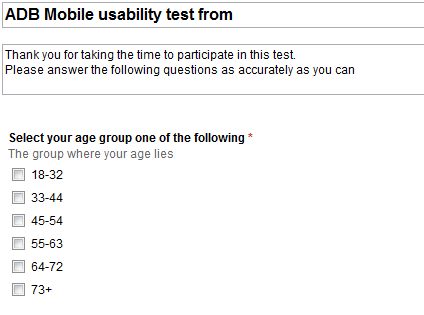
\includegraphics[width=1.0\textwidth]{ut_pic/1.png}
    \label{label: Usability test form item 1}
\end{figure}
\newpage
\begin{figure}[htb]
    \centering
    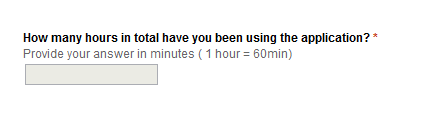
\includegraphics[width=1.0\textwidth]{ut_pic/4.png}
    \label{label: Usability test form item 1}
\end{figure}

\begin{figure}[htb]
    \centering
    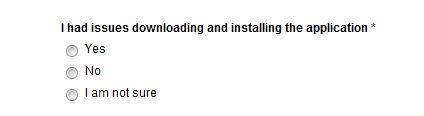
\includegraphics[width=1.0\textwidth]{ut_pic/3.png}
    \label{label: Usability test form item 1}
\end{figure}

\begin{figure}[htb]
    \centering
    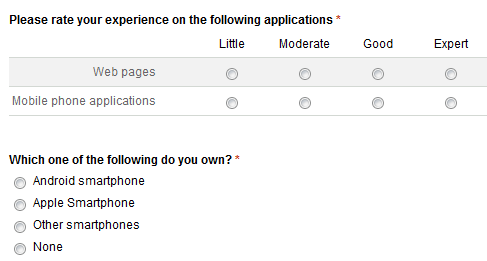
\includegraphics[width=1.0\textwidth]{ut_pic/2.png}
    \label{label: Usability test form item 1}
\end{figure}
\newpage 
